\experiment{Stack}{04/10/2023}

\section{Aim}
Write a menu driven C Program to implement a Stack using arrays with the operations:
\\1. Pushing elements to the Stack.
\\2. Popping elements from the Stack
\\3. Display the contents of the Stack after each operation


\section{Algorithm}
 {\fontfamily{lmtt}\selectfont

  \subsection{Create Stack}
  \begin{enumerate}[label=\arabic*:,left=0pt]
    \item \textbf{Start}

    \item Define a structure for a stack:
          \begin{enumerate}[label=2.\arabic*.]
            \item Include \texttt{top}, \texttt{size}, and an integer array \texttt{arr[100]}.
          \end{enumerate}

    \item Create a function \texttt{createStack()}:
          \begin{enumerate}[label=3.\arabic*.]
            \item Allocate memory for a new stack \texttt{s}.
            \item Set \texttt{s->top} to -1 and \texttt{s->size} to 100.
          \end{enumerate}
    \item Return \texttt{s}.
    \item \textbf{Stop}
  \end{enumerate}

  \subsection{Push Function}
  Create a function \texttt{push(s, data)}:
  \begin{enumerate}
    \item \textbf{Start}
    \item Check if \texttt{s->top} is equal to \texttt{s->size - 1}:
          \begin{enumerate}[label=2.\arabic*.]
            \item Print "Stack Overflow" and return.
          \end{enumerate}
    \item Increment \texttt{s->top}.
    \item Set \texttt{s->arr[s->top]} to \texttt{data}.
    \item \textbf{Stop}
  \end{enumerate}

  \subsection{Pop Function}
  Create a function \texttt{pop(s)}:
  \begin{enumerate}[label=\arabic*:,left=0pt]
    \item \textbf{Start}
    \item Check if \texttt{s->top} is less than 0:
          \begin{enumerate}[label=2.\arabic*:]
            \item Print "Stack Underflow" and return.
          \end{enumerate}
    \item Print "Removed element =", \texttt{s->arr[s->top]}.
    \item Decrement \texttt{s->top}.
    \item \textbf{Stop}
  \end{enumerate}

  \subsection{TOS Function}
  Create a function \texttt{tos(s)}:
  \begin{enumerate}[label=\arabic*:]
    \item \textbf{Start}
    \item Check if \texttt{s->top} is less than 0:
          \begin{enumerate}[label=2.\arabic*:]
            \item Print "Stack is empty" and return.
          \end{enumerate}
    \item Print "TOS =", \texttt{s->arr[s->top]}.
    \item \textbf{Stop}
  \end{enumerate}

  \subsection{Display Function}
  Create a function \texttt{display(s)}:
  \begin{enumerate}[label=\arabic*:]
    \item \textbf{Start}
    \item Loop from \texttt{s->top} to 0
          \begin{enumerate}[label=2.\arabic*:]
            \item Print \texttt{s->arr[i]}, followed by a space.
          \end{enumerate}
    \item Print a newline.
    \item \textbf{Stop Display Function}
  \end{enumerate}

  \subsection{Main Function}
  In the \texttt{main} function:
  \begin{enumerate}[label=\arabic*:, start=1]
    \item \textbf{Start}
    \item Create a stack \texttt{s} using \texttt{createStack()}.
    \item Initialize \texttt{ch}.
    \item \textbf{Start Menu Loop}
          \begin{enumerate}[label=4.\arabic*:, start=1]
            \item Print menu options.
            \item Take user input for \texttt{ch}.
            \item If \texttt{ch} is 1:
                  \begin{enumerate}[label=4.1.\arabic*:, start=1]
                    \item Take user input for \texttt{x}.
                    \item Call \texttt{push(s, x)}.
                  \end{enumerate}
            \item If \texttt{ch} is 2, call \texttt{pop(s)}.
            \item If \texttt{ch} is 3, call \texttt{tos(s)}.
            \item If \texttt{ch} is 4, call \texttt{display(s)}.
            \item If \texttt{ch} is 5, exit the loop.
            \item If \texttt{ch} is none of the above, print "Invalid option!".
          \end{enumerate}
    \item \textbf{Stop Menu Loop}
    \item \textbf{Stop}
  \end{enumerate}
 }



\section{C Program}
\begin{lstlisting}[label={list:c_program:stack}]
#include <stdio.h>
#include <stdlib.h>

typedef struct stack
{
  int top;
  int size;
  int arr[100];
} stack;

stack *createStack();
void push(stack *s, int data);
void pop(stack *s);
void tos(stack *s);
void display(stack *s);

int main()
{
  stack *s = createStack();
  s->size = 100;
  s->top = -1;
  int ch;
  printf("1)Push\n2)Pop\n3)tos\n4)Display\n5)Exit\n");
  do
  {
    printf("Choice: ");
    scanf("%d", &ch);
    if (ch == 1)
    {
      int x;
      printf("\nEnter the data: ");
      scanf("%d", &x);
      push(s, x);
    }
    else if (ch == 2)
    {
      pop(s);
    }
    else if (ch == 3)
    {
      tos(s);
    }
    else if (ch == 4)
    {
      display(s);
    }
    else if (ch != 5)
    {
      printf("\nInvalid option!\n");
    }
  } while (ch != 5);
}

stack *createStack()
{
  stack *s = (stack *)malloc(sizeof(stack));
  s->top = -1;
  s->size = 100;
  return s;
}

void push(stack *s, int data)
{
  if (s->top == s->size - 1)
  {
    printf("Stack Overflow\n");
    return;
  }
  s->top++;
  s->arr[s->top] = data;
}

void pop(stack *s)
{
  if (s->top < 0)
  {
    printf("Stack underflow\n");
    return;
  }
  printf("\nRemoved element = %d\n", s->arr[s->top]);
  s->top--;
}

void tos(stack *s)
{
  if (s->top < 0)
  {
    printf("Stack is empty\n");
    return;
  }
  printf("\nTOS = %d\n", s->arr[s->top]);
}

void display(stack *s)
{
  printf("\n");
  for (int i = s->top; i >= 0; i--)
  {
    printf("%d ", s->arr[i]);
  }
  printf("\n");
}
\end{lstlisting}

\section{Output}
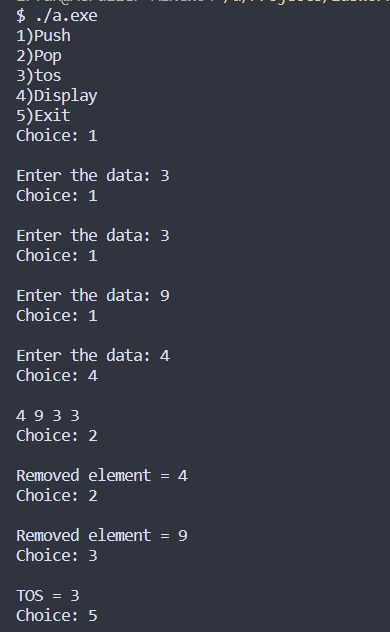
\includegraphics[]{Cycle_1/Outputs/Stack.png}

\section{Result}
Stack implemented using arrays. The program was executed and output verified.